\documentclass[a4paper,11pt]{book}
\usepackage[dutch]{babel}
\usepackage{textcomp}
\usepackage{fancyhdr}
\usepackage{makeidx}
\usepackage{tabularx}
\usepackage{graphicx}
\usepackage{parskip}
\usepackage{pdflscape}
\usepackage{floatflt}
\makeindex
\pagestyle{fancy}
\fancyhf{}
\fancyhead[LE,RO]{\bfseries\thepage}
\fancyhead[LO]{\bfseries\rightmark}
\fancyhead[RE]{\bfseries\leftmark}
\renewcommand{\headrulewidth}{0.5pt}
\renewcommand{\footrulewidth}{0pt}
\addtolength{\headheight}{0.5pt}
\fancypagestyle{plain}{%
	\fancyhead{}
	\renewcommand{\headrulewidth}{0pt}
}
\usepackage[pdfauthor={Rink Springer}
pdftitle={Plan van Aanpak}
pdftex]{hyperref}
%\hypersetup{colorlinks,citecolor=black,filecolor=black,linkcolor=black,urlcolor=black,pdftex}
\hyphenation{be-lang-rijk ont-wik-ke-laars me-taal-be-wer-king func-ti-o-na-li-teit}
\newcommand{\commsection}[1]{\subsection*{#1}}
\newcommand{\commsubsection}[1]{\subsubsection*{#1}}

% definities
\author{Rink Springer}
\title{Plan van Aanpak}

\begin{document}

\frontmatter

% titel pagina
\begin{titlepage}
\hrule
\vspace*{\fill}
\begin{center}
{\Huge Plan van Aanpak} \\
\vspace{2cm}
\begin{figure}[htb]
\begin{center}
\includegraphics[height=2cm]{delem_logo.jpg}
\end{center}
\end{figure}
HSB-Bus-Analyser\\
\vspace{2cm}
{\large Rink Springer}\\
\vspace{2cm}
Versie 1.31\\
\today\\
\vspace{2cm}
\end{center}
\vspace*{\fill}
\hrule
\end{titlepage}

% voorwoord
\section{Voorwoord}
\index{Voorwoord}

Dit Plan van Aanpak is geschreven tijdens mijn 2$^{e}$ stage bij de firma Delem. Het doel is de betrokkenen te informeren over mijn aanpak van het project en is in de eerste instantie bestemd voor mensen die in direct verband met de stage staan. Uiteraard is het ook voor ge\"interesseerden toegankelijk.

\index{Conclusie}
Ik wil iedereen die mij tijdens mijn stage geholpen heeft, heel erg bedanken. Hierbij in het bijzonder de heer M. Scholte, die mij als bedrijfsbegeleider op weg helpt binnen het bedrijf en de heer H. van Heumen, die als stagebegeleider namens Fontys Hogescholen te Eindhoven optreedt.


\tableofcontents

% samenvatting
\chapter{Samenvatting}
\index{samenvatting}

Dit verslag biedt een overzicht van mijn afstudeerstage bij Philips Research. Het directe resultaat is een Linux filesysteem dat direct in de Linux kernel opgenomen kan worden, programma's om het filesysteem aan te maken, te controleren en te debuggen. Tot slot is er een rapport geschreven dat de technische aspecten van het filesysteem belicht en een het uiteindelijke afstudeerverslag dat u nu aan het lezen bent.

Tijdens de stage heb ik erg diep in de Linux kernel gekeken, waarbij vooral de filesystemen en het I/O systeem centraal stond. Het resultaat hiervan is kennis over de interne Linux kernel structuren, die zeker van pas zullen komen in de toekomst. Verder heb ik ook de Extreme Programming-methode erg veel toegepast.


% verklarende woordenlijst
\thispagestyle{empty}
\chapter{Verklarende woordenlijst}
\index{Verklarende woordenlijst}
\label{woordenlijst}

\LTXtable{\textwidth}{woorden.tex}


\mainmatter

% 1. inleiding
\chapter{Inleiding}
\index{Inleiding}

Vlakbij Eindhoven Airport, aan de Luchthavenweg zit de firma Delem. Dit is een bedrijf dat zich richt op het ontwerpen en produceren van besturingen van drukpersen ten behoeve van metaalbewerking. Van februari tot juni 2004 heb ik stage gelopen bij de afdeling Development.

Er werken ongeveer 60 mensen bij Delem, waarvan ongeveer 30 in de afdeling Development. De overige werknemers werken bij de productie, sales en ondersteunende
afdelingen.

Gezien Delem zich in een zeer gespecialiseerde markt bevind, is kwaliteit afleveren zeer belangrijk. Maar minstens zo belangrijk is het bewaken van deze kwaliteit. Dat is in principe de essentie van deze opdracht, die in hoofdstuk 2 op pagina \pageref{opdracht} verder beschreven zal worden.

Daarna zullen vervolgens de onderzoeken, het proces, de implementatie en uiteindelijk de conclusie volgen. Elk hoofdstuk geeft een kijk op een ander deel van de stage, waarbij de conclusie vanzelfsprekend een afsluitende kijk op het geheel geeft.


% 2. bedrijf
\section[Delem]{Het bedrijf Delem}

\index{Delem}Delem werd in 1976 opgericht door de heer H.J.M.M. van Doorne. Op het moment is dit bedrijf de technologische leider op de wereldmarkt in het gebied van besturingen voor metaalbewerkingsmachines. Dit succes komt tot stand door het gebruik van de meest recente techniek in de producten. Delem levert uitsluitend aan OEM\footnote{Original Equipment Manufacturer}-ers (dus de bedrijven die metaalbewerkingsmachines maken) en niet aan eindklanten.

Er zijn ongeveer 60 personen werkzaam bij Delem. Ongeveer 30 hiervan zijn ICT-ers met gemiddeld een WO niveau.

Delem is opgedeeld in een aantal \index{Afdelingen}afdelingen, waarbij de voornaamste development, solutions, \index{Afdelingen!productie}productie en \index{Afdelingen!sales}sales zijn. Uiteraard is er ook nog ondersteunend personeel aanwezig, maar hier wordt verder niet op ingegaan. Een organigram is te vinden op pagina \pageref{organigram}.

In de volgende paragrafen staat een overzicht van de afdelingen die tijdens de stage van belang zijn:

\subsection{Afdeling Development}

\index{Afdelingen!development}Deze afdeling is verantwoordelijk voor het ontwikkelen van nieuwe hard- en software (voor zowel de besturing als voor een PC) en het onderzoeken van nieuwe mogelijkheden voor de besturingen. Gezien de aard van de stage wordt deze dan ook bij deze afdeling uitgevoerd. Zoals tijdens de planning op bladzijde \pageref{planning} te zien is, is er ook tijd gereserveerd voor assistentie voor de andere activiteiten van deze afdeling.

\begin{landscape}
\subsection{Organigram}
\index{Organigram}
\label{organigram}

\begin{figure}[h]{}
\includegraphics[width=18cm,height=9cm]{organisatie.jpg}
\end{figure}

\end{landscape}

\newpage


% 3. achtergrondinformatie
% dit commando is nodig om 2 plaatjes in 1 tabel te duwen
\newcommand{\cegraphic}[2]{{\renewcommand{\arraystretch}{0}
			    \begin{tabular}{c}%
			     \vrule height 0pt width 0pt\\
			     \includegraphics[#1]{#2}\\
			     \vrule height 0pt width 0pt
			    \end{tabular}}}

\section[Achtergrond]{Achtergrondinformatie}
\label{achtergrondinfo}

\subsection{De pers}

Om een goede indruk van een \index{Drukpers}drukpers te krijgen, zijn hieronder wat plaatjes te zien van een pers met daarin een metalen plaat die gebogen wordt:

\begin{figure}[h]
\begin{tabular}{cc}
\cegraphic{height=5cm}{pers1.jpg}&
\cegraphic{height=5cm}{pers2.jpg}
\end{tabular}
\end{figure}

Zoals in de plaatjes boven te zien is, wordt een product\footnote{In de plaatjes de blauwe plaat} gebogen doordat de \index{Persbalk}\emph{persbalk} naar beneden beweegt. Hierdoor komt de \index{Stempel}\emph{stempel} tegen het product aan, die door de \index{Matrijs}\emph{matrijs} tegengehouden wordt. De plaat hiertussen verbuigt daardoor, hetgeen resulteert in een buiging. De \index{Vingers}\emph{vingers} ondersteunen hierbij het product, zodat het op zijn plaats blijft.

\subsection{De modules}
\label{module}
De persbalk en de vingers worden aangestuurd door zogenaamde \index{Module}modules, die via een CAN\footnote{Controller Area Network, Ook wel bekend als HSB-bus} door de \index{Besturing}besturing\footnote{Op de vorige pagina het kastje uiterst links} worden aangestuurd.

Een overzicht van de besturing met de modules:

\begin{figure}[h]
\includegraphics[width=6.5cm]{hsb.jpg}
\end{figure}

Deze stageopdracht richt zich op de DM modules, en niet op de besturing zelf. De modules zelf sturen bijvoorbeeld motoren aan, of staan in verbinding met sensoren.


% 4. project
\section{Het project}
\label{project}

\index{Project}

\subsection{Informatie vooraf}

\index{Project!informatie}

Delem besturingen communiceren met de zogenaamde \index{CAN}CAN-bus naar modulen. Een \index{Module}module kan bijvoorbeeld een motor aansturen, die er bijvoorbeeld voor zorgt dat de persbalk naar een bepaalde positie gaat.

\subsection{Organisatie}
\label{organisatie}

De \index{Opdrachtgever}opdrachtgever van het project is de firma Delem, die als stagebegeleider de heer M. Scholte heeft aangewezen.

De \index{Opdrachtnemer}opdrachtnemer is de heer R. Springer, student van Fontys Hogescholen te Eindhoven. De begeleidende docent is de heer H. van Heumen.

\subsection{Probleemstelling}

\index{Project!probleemstelling}
\label{probleemstelling}

Op het moment is er geen manier waarop modulen specifiek getest kunnen worden. Om nu een module te testen wordt er soms een compleet systeem gebouwd met besturing en motoren.

Aangezien dit niet praktisch is, hebben engineers zelf oplossingen bedacht om toch zoveel mogelijk lokaal te kunnen testen. Hierbij werd vooral de scripttaal \index{Perl}Perl\footnote{www.perl.com} gebruikt, samen met een hele hoop tooltjes.

\subsection{Resultaat}
\index{Project!resultaat}

De bedoeling is een programma te ontwikkelen dat modulen kan testen. Aangezien er nog onduidelijk is wat er het beste getest kan worden en welke CAN PC hardware het beste gebruikt kan worden, zal er eerst een \index{Analyse}analyse uitgevoerd worden om te kijken welke hardware het beste voldoet.

De functionaliteit die er absoluut in moet zitten, is het leesbaar weergeven van berichten op de CAN bus, alsmede de mogelijkheid om zelf berichten naar modulen te kunnen sturen. Dit kan niet met conventionele programma's, aangezien Delem zelf berichten toegevoegd heeft die niet in de CAN specificatie staan. Extra functionaliteit zal na de analyse en in de loop van het project toegevoegd worden.

\subsection{Randvoorwaarden}

De \index{Randvoorwaarden} randvoorwaarden van dit project zijn als volgt:

\begin{itemize}
\item Alle toegezegde middelen blijven beschikbaar tot het eind van de stageperiode.
\item Belanghebbenden van het project maken genoeg tijd beschikbaar voor ondersteuning van de stagiair.
\end{itemize}

\subsection{Risico's}
\index{Risico's}

Zoals bij elke stageopdracht is er het risico dat er niet genoeg kennis bij de stagiair aanwezig is, wat als resultaat heeft dat het project niet op tijd af komt. Aan de hand van de ervaring van de bedrijfsbegeleider en de kennis van de aanwezige ICT-ers bij het bedrijf en de stagiair zelf is de kans dat dit gebeurt klein.

\subsection{Fasering}

\label{fasering}
\index{Fasering}

Bij Delem wordt de doorlooptijd van projecten in zogenaamde \index{Milestones}\emph{milestones} verdeeld. Milestones worden weer onderverdeeld in zogenaamde \index{Increments}\emph{increments}, een periode van 2 weken. Hieronder is een overzicht te vinden van de milestones, inclusief hun rol met betrekking tot dit project:

\newpage
\subsubsection{Overzicht}

\label{faseringoverzicht}
\index{Fasering!overzicht}
\begin{figure}[h]
\includegraphics[width=\textwidth]{proces.jpg}
\end{figure}

\subsubsection{Toelichting}
\index{Fasering!toelichting}

Hieronder volgt een toelichting van de fasering, zoals die in het plaatje hierboven te zien is:

\begin{itemize}
\item Milestone 0: Studie\\
Het doel hier is het project te defini\"eren. De uitkomst hiervan is normaal gesproken een commerci\"ele beschrijving, zoals wat er nu in \index{SAIS}SAIS\footnote{Fontys' Stage- en Afstudeer Informatie Systeem, zie http://intranet.hi.fontys.nl/sais} te vinden is. Dit wordt een CRS\footnote{Commercial Requirements Specification} genoemd.
\item Milestone 1: Voorbereiding\\
Tijdens deze fase wordt het product formeel voorbereid. Hierbij worden vooral zaken geanalyseerd. Het hoofdstuk planning op bladzijde \pageref{planning} in dit Plan van Aanpak wordt uitgebreid aan de hand van de bevindingen hiervan. Het directe resultaat is het Plan van Aanpak. Dit wordt een \index{URD}URD\footnote{User Requirements Document} genoemd.
\item Milestone 2: Ontwerp\\
In deze fase wordt het product echt ontworpen. Als het een hardwareproduct is worden de schema's ontwikkeld, bij softwareproducten worden hier bijvoorbeeld de \index{UML}UML\footnote{Universal Modelling Language} schema's getekend.
\item Milestone 3: Implementatie en testen\\
Nu wordt het product daadwerkelijk gemaakt. De bedoeling is dat aan het eind van deze milestone een prototype van het product af is.

Het product wordt tijdens het implementeren ook getest door de ontwikkelaars zelf. Dit resulteert in CR's en PR's, hier zal later op worden ingegaan.
\item Milestone 4: Product test release\\
Hier wordt het product vrijgegeven voor interne release, waar het ook uitgebreid getest gaat worden door de testafdeling. Dit resulteert in nog meer CR's en PR's.
\end{itemize}

Aangezien dit een product voor intern gebruik is, zijn milestone 5: Markt release, milestone 6: Project sluiting en milestone 7: onderhoud weggelaten. De uiteindelijke planning is te vinden op bladzijde \pageref{planning}.

Op de volgende pagina is een overzicht te zien van de projectplanning zoals deze bij Delem gehanteerd wordt:

\subsection{Hulpprogramma's}

\index{Hulpprogramma's}

Er wordt bij Delem gebruikt gemaakt van een drietal programma's, waarmee de bronnen in een project en de status ervan goed bewaakt kunnen worden. Deze programma's zijn:

\begin{itemize}
\index{Primavera!Project Manager}
\item Primavera Project Manager\\
Met dit programma kunnen alle activiteiten omtrent een project ingepland worden. Via \index{Primavera!Progress Reporter}Primavera Progress Reporter kunnen mensen die aan het project werken uren boeken op deze activiteiten. Zo is meteen te zien hoeveel uur ergens voor ingepland werd en hoeveel tijd er daadwerkelijk aan besteed is.
\index{PVCS!Tracker}
\item PVCS Tracker\\
Dit programma slaat de CR's en PR's op in een database, waarop gezocht kan worden. Elke CR en PR heeft een eigenaar, die verantwoordelijk is voor de request. Opmerkingen en dergelijke kunnen bij de CR en PR gevoegd worden, zodat er altijd een goed overzicht is wat de status en geschiedenis van de request is.
\index{PVCS!Version Manager}
\item PVCS Version Manager\\
Dit programma is vergelijkbaar met CVS\footnote{Concurrent Version System, zie www.cvs.org} of diens voorganger RCS\footnote{Revision Control System}. Alle projectbestanden worden hiermee onder versiebeheer geplaatst. Dit zorgt ervoor dat alle veranderingen tot de projectbestanden, of dat nu broncode, documentatie of wat dan ook is, altijd gearchiveerd word.
\end{itemize}

\subsubsection{CR's en PR's}

\index{CR}
\index{PR}
\label{PR}
\label{CR}

Zoals in de vorige paragraaf al naar voren kwam, zijn PR\footnote{Problem Report}'s en CR\footnote{Change Request}'s erg belangrijk. Deze twee zaken kunnen worden gecr\"eerd en opgezocht worden met behulp van de PVCS Tracker.

Het doel hiervan is een duidelijk overzicht te hebben van de taken die voor het project uitgevoerd moeten worden. Verder kan er met behulp van de Progress Reporter aangegeven worden hoeveel tijd er daadwerkelijk gespendeerd is aan een taak, zodat er meteen een duidelijk overzicht is.

\subsubsection{Change Control Board}
\index{CCB}
\label{CCB}
CR's en PR's worden beheerd door middel van een CCB\footnote{Change Control Board}. Als een CR/PR is ingeschoten, dan besluit normaal gesproken het CCB (dit is normaal gesproken een team van de projectleider, projectleden en sales/management personen) of die CR/PR wel of niet gehonoreerd wordt.

\subsection{Analyses}

De volgende analyses zullen worden uitgevoerd:

\begin{itemize}
\item \index{Analyse!hardware}Hardware analyse \\
Het doel van deze analyse is om uit te zoeken wat de beste hardware is om met de modulen te communiceren.
\item \index{Analyse!functionaliteit}Functionaliteit analyse \\
Deze analyse concentreert zich op de functionaliteit die het programma moet krijgen. Om dit te doen zullen de mensen die veel met DM modulen te maken hebben, naar hun mening hierover gevraagd worden. Aan de hand hiervan zal er samen met de bedrijfsbegeleider een overzicht gemaakt worden van functionaliteit die erin moet zitten, functionaliteit die gewenst is en functionaliteit die niet noodzakelijk is.
\end{itemize}


% 5. planning
\section{Planning}

Dit hoofdstuk zal een overzicht van de planning geven. Op de volgende bladzijde is een overzicht van de planning te zien, dat daarna toegelicht zal worden.

\begin{landscape}
\subsection{Overzicht}
\index{Planning!overzicht}

\begin{figure}[h]
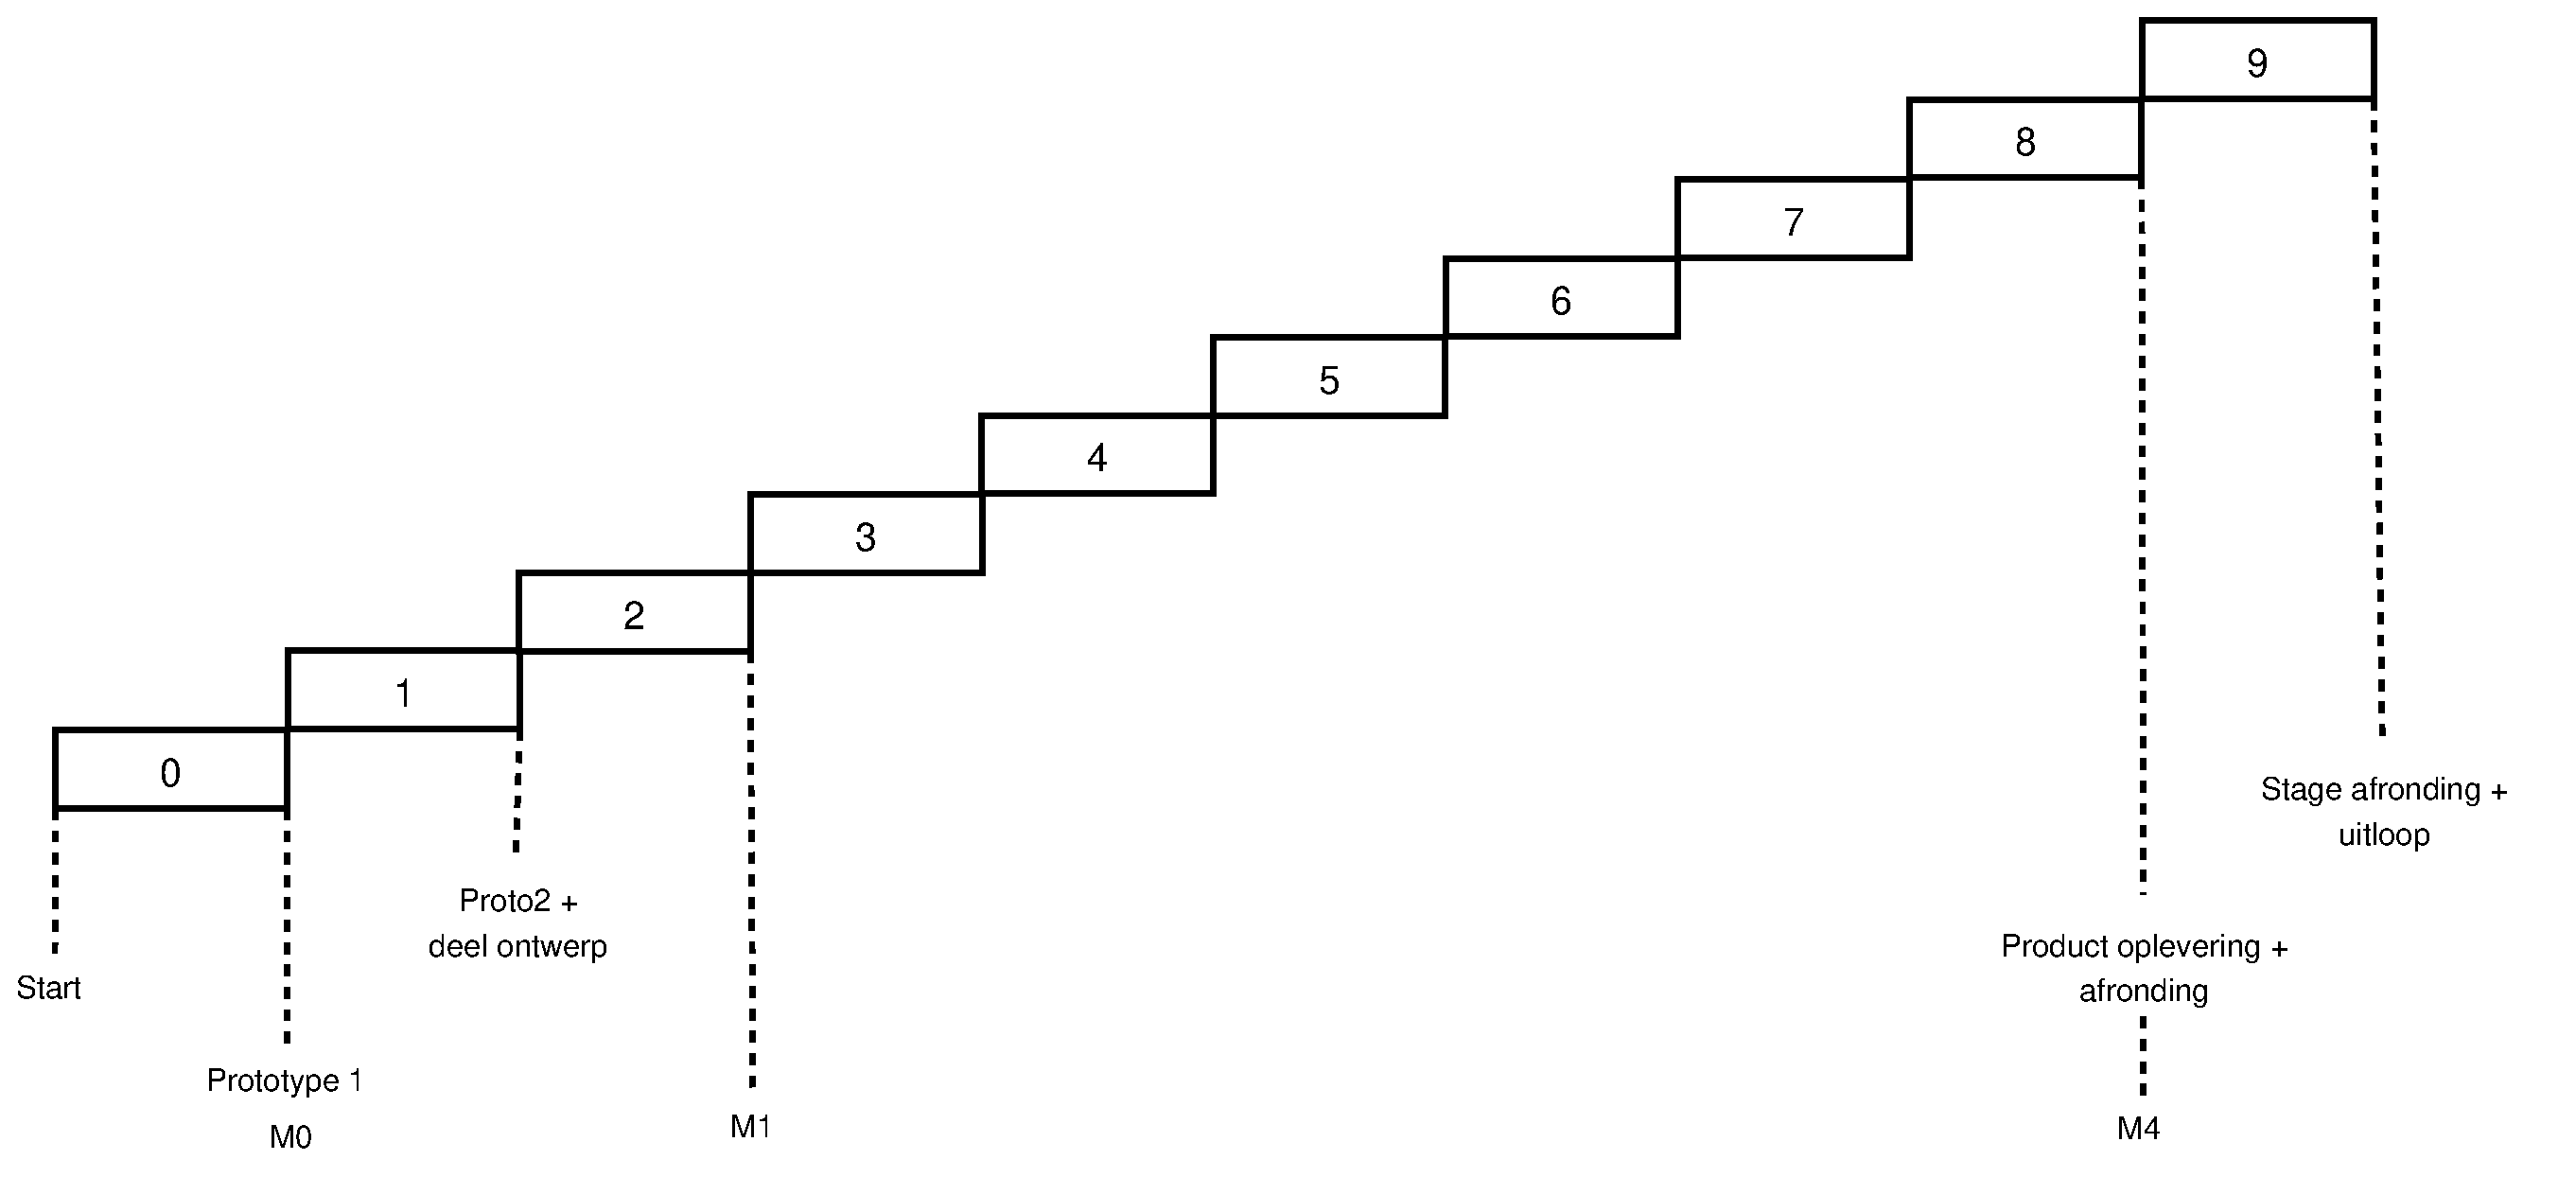
\includegraphics[width=20cm]{planning}
\end{figure}

In dit schema geven de rechthoekige genummerde vakken de increments aan. De gestippelde lijnen geven de gepland afgeronde activiteiten aan en de geplande milestones.

\end{landscape}

\newpage
\subsection{Toelichting}
\index{Planning,toelichting}
\label{planning}

Zoals in de fasering op bladzijde \pageref{fasering} besproken werd, wordt het project ingedeeld in \index{Milestones}milestones. Deze zijn zelf weer opgedeeld in \'e\'en of meerdere \index{Increments}increments.

\begin{tabularx}{\textwidth}{|c|c|X|}
\hline
Increment&Datum&Activiteit\\
\hline
0&2 - 13 Februari&Opstellen en aanpassen Plan van Aanpak, analyses uitvoeren, prototype1\\
\hline
\multicolumn{3}{|l|}{\textbf{Milestone 0: Studie}}\\
\hline
%\hline
%\multicolumn{3}{|l|}{\textbf{Milestone 2: Ontwerp}}\\
%\hline
1&16 - 27 Februari&Prototype2 + deel ontwerp\\
2&1 - 12 Maart&\\
\hline
\multicolumn{3}{|l|}{\textbf{Milestone 1: Voorbereiding}}\\
\hline
3&15 - 26 Maart&\\
%\hline
%\multicolumn{3}{|l|}{\textbf{Milestone 3: Implementatie en testen}}\\
%\hline
4&29 Maart - 9 April&\\
5&12 - 23 April&\\
6&26 April - 7 Mei&\\
7&10 - 21 Mei&\\
8&24 Mei - 4 Juni&Afronden en opleveren product\\
\hline
\multicolumn{3}{|l|}{\textbf{Milestone 4: Product test release}}\\
\hline
9&7 - 18 Juni&Stage afronden, presentatie houden, stageverslag maken\\
\hline
\end{tabularx}

Zoals tijdens de probleemstelling (zie pagina \pageref{probleemstelling}) te zien is, zal al lopende het project extra functionaliteit aangedragen worden. Deze planning zal dan ook aangepast worden.

Het faseringsoverzicht op pagina \pageref{faseringoverzicht} laat zien dat de milestones door elkaar heen lopen. Daarom zijn milestone 2: ontwerp en milestone 3: implementatie en testen niet in deze planning opgenomen.

Tenslotte wil Delem dat ik maximaal \'e\'en dag in de week reserveer voor zaken die niet direct in verband staan met de HSB Bus Analyser, maar waar ik bijvoorbeeld Solutions werk ga doen. Dit omdat er tijdens het werken in een bedrijfssituatie regelmatig iets tussendoor komt wat hogere prioriteit heeft.


% 6. beheersaspecten
\section{Beheersaspecten}

\subsection{Geld}

Delem stelt een maandelijkse stagevergoeding beschikbaar, deze bedraagt \texteuro 406,92 bruto per maand. Verder zal er ook de mogelijkheid om in overleg benodige zaken te kopen.

\subsection{Organisatie}

Zie projectorganisatie op pagina \pageref{organisatie}.

\subsection{Kwaliteit}

In de eerste instantie zal het product zoveel mogelijk door de stagiair zelf getest worden tijdens het ontwikkelen, dit is gebruikelijk binnen Delem. Als de eerste release van het programma vrijgegeven wordt, zullen de gebruikers van het programma hun bevindingen melden, en er indien nodig een PR of CR van maken.

\subsection{Informatie}

Er zal om de week een overleg zijn met de bedrijfsbegeleider, alswel een tweewekelijkse rapportage naar de docentbegeleider.

De software voor het te maken project zal geschreven worden in Microsoft Visual C++ .NET, en moet werken op Windows 2000 en XP machines.

\subsection{Tijd}

De stage duurt tot 18 juni 2004. Op dit tijdstip moet het project afgerond zijn en aan alle formaliteiten voldaan zijn. In geval van ziekte en andere onvoorziene zaken is er eventueel \'e\'en week extra.


% 7. conclusie / aanbevelingen
\chapter{Conclusie}
\index{Conclusie}

Dit verslag bied een overzicht van het verloop van mijn werkzaamheden tijdens mijn $2^e$ stage te Delem BV. Na het gehele verloop van de stage is er een programma gemaakt, waarvan ik hoop dat Delem er veel aan zal hebben. De opzet was het programma zo uitbreidbaar en onderhoudbaar mogelijk te maken, iets wat goed gelukt is.

Tijdens deze stage heb ik, behalve aan de stageopdracht te werken, ook ongeveer \'e\'en dag per week aan andere activiteiten besteed. Een goed voorbeeld hiervan is het testen van een bestaande applicatie VBend\footnote{Virtual Bend, applicatie die een optimale buigvolgorde kan berekenen en simuleren}, waarvan binnenkort een nieuwe versie beschikbaar zou komen. Hierbij ben ik volledig in het projectteam opgenomen en heb ik goed kennis leren maken met de gang van zaken tijdens 'normale' projecten. Ook kwam het gebruik van \index{PR}PR's en \index{CR}CR\footnote{Problem Report/Change Request, zie pagina \pageref{PR} voor meer informatie}'s erg goed naar voren.

Verder heb ik tijdens deze stage heel uitgebreid kennis gemaakt met XML, wat wellicht later nog van pas kan komen. Ook merkte ik dat mijn Windows programmeerkennis niet meer optimaal was (ik gebruik zelf thuis bijna geen Windows), daarin heb ik mezelf ook een stuk meer verdiept.

Ik vind dat ik veel vrijheid heb gehad tijdens het uitoefenen van de stage, ik verwacht dat dit is omdat ik inmiddels al 2 jaar bij de firma Delem werkzaam ben. Hierbij ben ik van mening dat ik nu pas het bedrijf echt goed heb leren kennen, gezien ik eigenlijk pas nu het gevoel heb dat ik weet hoe de projecten daar werken .

Tenslotte denk ik dat dit een geslaagde stage was. Het is goed gedocumenteerd, er is een goed functionerend programma opgeleverd en er zijn al een aantal problemen mee gevonden die wellicht in de toekomst aangepakt zullen worden. Al met al een prima resultaat, wat ook door mijn projectbegeleider bij Delem bevestigd is.


% communicatieplan
\appendix
\chapter{Communicatieplan}

Deze bijlage bevat het communicatieplan, zoals uiteindelijk met de docentbegeleider overeen gekomen. Uiteindelijk bleek het stageverslag eerder af te zijn dan gepland en word daarom ook eerder opgestuurd.

% communicatieplan
\chapter{Communicatieplan}

Deze bijlage bevat het communicatieplan, zoals uiteindelijk met de docentbegeleider overeen gekomen. Uiteindelijk bleek het stageverslag eerder af te zijn dan gepland en word daarom ook eerder opgestuurd.

% communicatieplan
\chapter{Communicatieplan}

Deze bijlage bevat het communicatieplan, zoals uiteindelijk met de docentbegeleider overeen gekomen. Uiteindelijk bleek het stageverslag eerder af te zijn dan gepland en word daarom ook eerder opgestuurd.

% communicatieplan
\input{commplan/commplan.tex}




% index
\backmatter
\printindex

\end{document}
